\PassOptionsToPackage{expansion=false}{microtype}
\documentclass[manuscript,review,anonymous]{acmart}
\usepackage{tabularx}
\usepackage{ragged2e}
\newcolumntype{L}{>{\RaggedRight\arraybackslash}X}
\usepackage{booktabs}
\usepackage{float}
\usepackage{tikz}
\usetikzlibrary{shapes.geometric, arrows.meta, positioning, calc, fit, backgrounds}

\tikzset{
    block/.style={rectangle, draw, fill=blue!5, text width=6em, text centered, rounded corners, minimum height=3em, font=\small},
    subblock/.style={rectangle, draw, fill=gray!10, text width=5em, text centered, rounded corners, minimum height=2.5em, font=\footnotesize},
    io/.style={trapezium, trapezium left angle=70, trapezium right angle=110, draw, fill=green!5, text width=4em, text centered, minimum height=2em, font=\small},
    cloud/.style={draw, ellipse, fill=red!5, text width=6em, text centered, minimum height=3em, font=\small},
    decision/.style={diamond, draw, fill=yellow!5, text width=4.5em, text centered, inner sep=0pt, font=\footnotesize},
    arrow/.style={thick, ->, >=stealth},
    phase/.style={rectangle, draw, dashed, inner sep=0.3cm, font=\bfseries\small}
}
%%
%% \BibTeX command to typeset BibTeX logo in the docs
\AtBeginDocument{%
  \providecommand\BibTeX{{%
    Bib\TeX}}}

% \setcopyright{acmlicensed}
% \copyrightyear{2018}
% \acmYear{2018}
% \acmDOI{XXXXXXX.XXXXXXX}
% \acmISBN{978-1-4503-XXXX-X/2018/06}

\usepackage{pgfplots}
\pgfplotsset{compat=1.18}

%%
%% end of the preamble, start of the body of the document source.
\begin{document}

%%
%% The "title" command has an optional parameter,
%% allowing the author to define a "short title" to be used in page headers.
\title{Towards Fair Fares: Designing a Resilient Contactless Payment Ecosystem for Public Transit in Nepal}

\author{Prashant Adhikari}
\email{prashant_adhikari_a25@sunway.edu.np}
\orcid{0009-0008-6960-7907}
\affiliation{%
  \institution{Sunway College Kathmandu}
  \city{Kathmandu}
  \state{Bagmati}
  \country{Nepal}
}

\author{Maladeep Upadhyaya}
\email{maladeep@sunway.edu.np}

\affiliation{%
  \institution{Sunway College kathmandu}
  \city{Kathmandu}
  \state{Bagmati}
  \country{Nepal}}

\author{Supriya Khadka}
\email{skhadk@gmu.edu}
\affiliation{%
  \institution{George Mason University}
  \city{Fairfax}
  \state{Virginia}
  \country{USA}}

%%
%% By default, the full list of authors will be used in the page
%% headers. Often, this list is too long, and will overlap
%% other information printed in the page headers. This command allows
%% the author to define a more concise list
%% of authors' names for this purpose.
\renewcommand{\shortauthors}{Adhikari et al.}

%%
%% The abstract is a short summary of the work to be presented in the
%% article.
\begin{abstract}
Urban mobility in rapidly growing Nepali cities like Kathmandu and Pokhara is severely constrained by a persistent reliance on cash-based fare collection. Recent efforts to digitize public transit using general-purpose QR code wallets (such as \textit{eSewa} and \textit{Khalti}) have inadvertently introduced new infrastructural frictions. These mobile-first solutions often fail in the dynamic environment of a moving vehicle, where scanning delays and dropped cellular signals exacerbate boarding bottlenecks. To bridge this socio-technical gap, we introduce TransitPay, an equitable, offline-capable payment ecosystem using Near Field Communication (NFC) and Host Card Emulation (HCE). By intentionally designing around affordable hardware (ESP8266 and PN532) and utilizing a local data queuing architecture, the system processes transactions independently of real-time cloud connectivity. Importantly, shifting the internet requirement exclusively to the vehicle's Point-of-Sale terminal removes the burden of mobile data access from the commuter. Sandboxed evaluations demonstrate that TransitPay reduces transaction latency from a typical 30 seconds to just 1.5 to 2.5 seconds. This 94 percent reduction in wait time represents more than a technical optimization; it represents a major step toward an inclusive, resilient transit infrastructure designed specifically for the realities of the digital age.
\end{abstract}

%%
%% The code below is generated by the tool at http://dl.acm.org/ccs.cfm.
%% Please copy and paste the code instead of the example below.
%%
\begin{CCSXML}
  <ccs2012>
     <concept>
         <concept_id>10010405.10010481.10010485</concept_id>
         <concept_desc>Applied computing~Transportation</concept_desc>
         <concept_significance>500</concept_significance>
         </concept>
     <concept>
         <concept_id>10010520.10010553</concept_id>
         <concept_desc>Computer systems organization~Embedded and cyber-physical systems</concept_desc>
         <concept_significance>500</concept_significance>
         </concept>
     <concept>
         <concept_id>10003120.10003138.10003140</concept_id>
         <concept_desc>Human-centered computing~Ubiquitous and mobile computing systems and tools</concept_desc>
         <concept_significance>300</concept_significance>
         </concept>
   </ccs2012>
\end{CCSXML}
  
\ccsdesc[500]{Applied computing~Transportation}
\ccsdesc[500]{Computer systems organization~Embedded and cyber-physical systems}
\ccsdesc[300]{Human-centered computing~Ubiquitous and mobile computing systems and tools}


%%
%% Keywords. The author(s) should pick words that accurately describe
%% the work being presented. Separate the keywords with commas.
\keywords{Urban Mobility, Digital Equity, Contactless Transit, Offline-First Architecture, Host Card Emulation}
%% A "teaser" image appears between the author and affiliation
%% information and the body of the document, and typically spans the
%% page.

% \received{20 February 2007}
% \received[revised]{12 March 2009}
% \received[accepted]{5 June 2009}

%%
%% This command processes the author and affiliation and title
%% information and builds the first part of the formatted document.
\maketitle

\section{Introduction}
Consider a commuter navigating a crowded microbus in Kathmandu.  In a valley where over 90\% of the public transit fleet consists of low-capacity minibuses and microbuses, the conductor must squeeze through a packed aisle to collect physical currency~\cite{jica2017kathmandu_transport,aryal2022strong}. This manual process routinely leads to fare disputes and severe revenue leakage, with reports indicating that conductors often hand over only half of their actual daily collections to vehicle owners~\cite{annapurnaexpress2026article}. Because Nepal's public transit remains almost entirely dependent on cash, the entire urban mobility network suffers from severe boarding bottlenecks. When the payment process stalls, the daily dignity and economic mobility of the 28\% of valley residents who rely on this infrastructure are significantly restricted~\cite{jica2017kathmandu_transport}.

While digital wallets like \textit{eSewa} and \textit{Khalti} have successfully modernized retail in Nepal, public transit presents a uniquely hostile environment for standard mobile payments. The core issue is severe boarding latency. Commuters attempting to scan a QR code face transaction times that can drag on for up to 30 seconds. More critically, these mobile-first systems require continuous cellular data and completely fall apart when a moving vehicle enters a network blind spot~\cite{gupta2022m}. Because Nepal's broadband infrastructure is highly inconsistent, these digital attempts often fail, forcing commuters and conductors back to manual cash handling.

Previous attempts to digitize transit fares in the region have recognized the need for faster technologies but have seen limited success. Initiatives like Sajha Yatayat's smart cards~\cite{annapurnaexpress2026article} and the Yatra Card~\cite{fintech2023yatra} introduced NFC technology for a faster tap-in and tap-out experience. However, these implementations operate strictly as closed-loop systems. A proprietary card for one bus network cannot be used on a private microbus, failing to solve the interoperability gap. Furthermore, while the National Payment Switch integrates retail wallets, it currently lacks a standardized API for cross-operator transit fare settlement.

To bridge this socio-technical gap, we detail the development of TransitPay, an equitable, offline-capable payment ecosystem built using Near Field Communication (NFC) and Host Card Emulation (HCE). By intentionally designing around simple, affordable hardware, specifically the ESP8266~\cite{esp8266soc} and PN532~\cite{nxp2016pn532}, we created a system that shifts the internet requirement exclusively to the vehicle's Point-of-Sale terminal. Utilizing a local data queuing architecture, the system processes transactions securely offline and synchronizes with the cloud only when the vehicle regains cellular range. To ensure economic fairness, the system also integrates a GPS module to track boarding and alighting coordinates automatically.

This work is guided by two primary research questions:
\begin{itemize}
  \item \textbf{RQ1}: How can an offline-first NFC architecture reduce boarding latency and improve payment resilience in resource-constrained transit environments?

  \item \textbf{RQ2}: How does an automated, location-based payment model impact the transparency and economic fairness of fare collection for daily commuters?
\end{itemize}

To address these questions, we offer three main contributions to the field of sustainable urban computing:
\begin{itemize}
  \item The design and implementation of TransitPay, an affordable (NPR 3000) IoT hardware architecture tailored specifically to bypass intermittent internet connectivity via local data queuing.
  \item The introduction of a ``Fair Fare Model'' that utilizes onboard GPS coordinates to automatically calculate distance-based pricing, eliminating manual revenue leakage and protecting passengers from arbitrary overcharging.
  \item Sandboxed empirical evaluations demonstrating that this system achieves a best-case transaction speed of 1.5 to 2.5 seconds, reducing wait times by 94 percent compared to existing QR methods.
\end{itemize}


\section{Related Works}

\subsection{Digital Fare Collection in the Global South}
Across the Global South, public transportation frequently relies on decentralized, semi-formal fleets like minibuses, jeepneys, or matatus~\cite{jica2017kathmandu_transport}. The transition from cash-based fare collection to digital payment ecosystems in these environments presents many infrastructural challenges. While QR code payments have historically dominated the broader retail sectors in large markets such as India and China~\cite{}, deploying these optical systems in dynamic, moving transit environments often introduces bottlenecks~\cite{}.

Currently, there is a notable shift toward NFC technologies in developing regions to address these frictions. Southeast Asia is experiencing a massive surge in NFC adoption, with countries like the Philippines, Thailand, and Vietnam projected to reach 75 percent digital wallet penetration by late 2026~\cite{juniper2022digital}. As these nations attempt to integrate digital payments into their transit networks, direct comparisons between QR and NFC methods have become vital. Research on mobile fare payment systems shows that QR-code ticketing can increase boarding service time due to scanning procedures and recognition delays, sometimes causing crowding at transit entry points, whereas NFC-based ``tap-and-go'' systems validate transactions in around 100-120 ms and enable faster passenger throughput~\cite{chen2020influence}.

\subsection{The Offline-First Imperative for Financial Inclusion}
A core challenge in deploying transit fintech in the Global South is the assumption of continuous, ubiquitous internet connectivity. Many modern mobile wallets rely entirely on real-time cloud authorization to process transactions~\cite{}. This design choice inherently introduces friction in resource-constrained environments, creating a barrier to true financial inclusion for users who cannot afford consistent mobile data plans or who are traveling through network dead zones. In Nepal, for instance, weak last-mile connectivity and patchy broadband heavily restrict the reliability of real-time cloud payments on moving vehicles~\cite{kharel2025digital}. 

To combat infrastructural fragility, researchers in Information and Communication Technology for Development (ICTD) increasingly advocate for ``offline-first'' architectures~\cite{}. By localizing data processing to the edge device, systems can ensure transaction resilience even when the broader network fails~\cite{}. TransitPay integrates this philosophy directly into its hardware and software design. By utilizing a local data queuing method on the ESP8266 microcontroller, the system deliberately shifts the connectivity burden away from the commuter's smartphone and onto the vehicle's Point-of-Sale terminal. This localized processing ensures that digital public goods remain accessible, equitable, and functional, regardless of fluctuating cellular signals.

\subsection{Digital Transit Infrastructure in Nepal}

To address these global challenges locally, recent initiatives in Nepal have attempted to digitize urban transit using Near Field Communication (NFC). NFC is a short-range wireless technology that enables secure, instant data exchange between active and passive devices separated by just a few centimeters, making it the standard for frictionless ``tap-and-go'' payments~\cite{singh2020near}. In Kathmandu, operators like Sajha Yatayat and Fintech International have introduced NFC-enabled smart cards (such as the Yatra Card) to calculate distance-based fares and reduce revenue leakage~\cite{fintech2023yatra, annapurnaexpress2026article}. 

However, these solutions operate strictly as closed-loop systems. A proprietary card issued for one network cannot be utilized on a private microbus, failing to solve the interoperability gap for the average commuter, especially since the National Payment Switch currently lacks a standardized transit API~\cite{nrb2025paymentoversight}. To bypass this fragmentation, commuters frequently attempt to use ubiquitous mobile wallets (such as \textit{eSewa} or \textit{Khalti}) that rely on QR codes. Unfortunately, direct comparisons reveal that manual QR scanning in dynamic transit environments routinely takes over 10 seconds, causing severe passenger stacking at bus doors~\cite{chen2020influence}. Furthermore, because these mobile-first systems lack offline data queuing, they frequently fail when moving vehicles cross network blind spots~\cite{kharel2025digital}. 

TransitPay builds upon these foundational efforts by utilizing Host Card Emulation (HCE) to emulate NFC cards via software~\cite{alattar2014host, alliance2014host}. This approach merges the interoperability of a mobile application with the offline resilience and speed of a physical NFC smart card, engineering a solution specifically tailored for Nepal's fragmented and connectivity-constrained transit ecosystem.

\section{Methodology}

In this section, we will outline the methodology we approached to design and develop our proposed system that works as the payment service provider for the public transit in metro cities of Nepal.  While various engineering design methodologies exist, ranging from the software-centric Agile framework used for rapid application iteration to the hardware-focused V-Model for protocol verification, this research adopts a Systems Engineering Design Methodology. This approach is specifically chosen to harmonize the multi-layered complexity of the TransitPay ecosystem, ensuring seamless integration between the IoT hardware (ESP8266/PN532), the HCE-enabled React Native mobile client, and the MongoDB-backed Node.js server. This section will be divided into seven distinct parts: system design, user flow pipeline, and cost breakdown.

\subsection{System Design}


The system design and architecture of the proposed system is secure with the communication of the NFC entity and the point of sale, with the POS sending APDU challenges to the NFC entity, and after the entity solves the APDU challenges, it sends the encrypted data using the entity’s unique private key; afterwards, the POS decrypts the data using the public key embedded in it, and then the communication between the NFC entity and the POS is successful. 


\begin{figure*}[t]
  \centering
  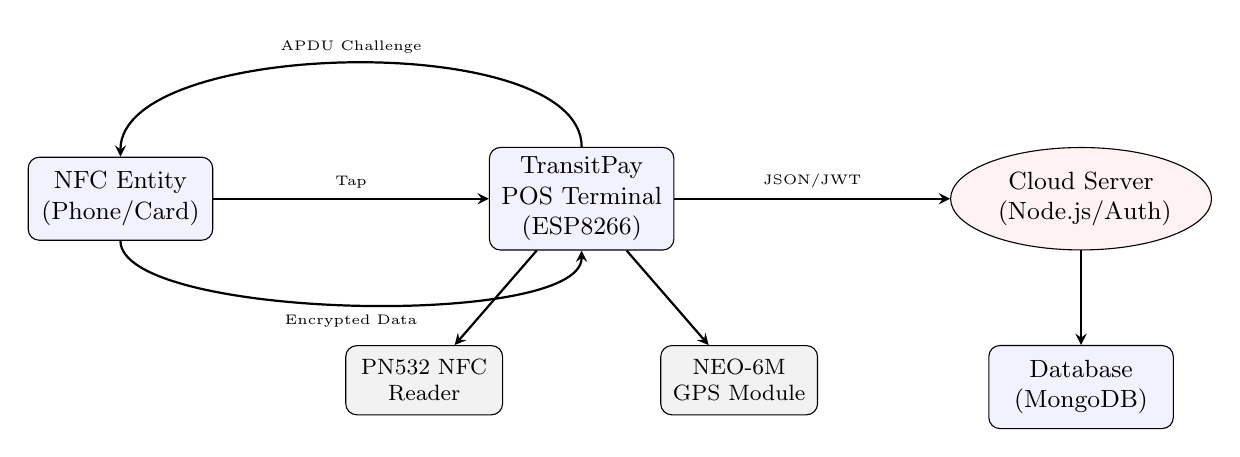
\begin{tikzpicture}[node distance=3.5cm]
    % Central POS
    \node (pos) [block] {TransitPay POS Terminal (ESP8266)};
    
    % Peripherals
    \node (entity) [block, left=of pos] {NFC Entity (Phone/Card)};
    \node (pn532) [subblock, below=1.2cm of pos, xshift=-2cm] {PN532 NFC Reader};
    \node (neo6m) [subblock, below=1.2cm of pos, xshift=2cm] {NEO-6M GPS Module};
    
    % Infrastructure
    \node (server) [cloud, right=of pos] {Cloud Server (Node.js/Auth)};
    \node (db) [block, below=1.2cm of server] {Database (MongoDB)};

    % Primary Flow
    \draw [arrow] (entity) -- node[above, font=\tiny] {Tap} (pos);
    \draw [arrow] (pos) -- (pn532);
    \draw [arrow] (pos) -- (neo6m);
    \draw [arrow] (pos) -- node[above, font=\tiny] {JSON/JWT} (server);
    \draw [arrow] (server) -- (db);
    
    % APDU Handshake (Curved to avoid overlapping)
    \draw [arrow] (pos.north) .. controls +(up:1.5cm) and +(up:1.5cm) .. node[above, font=\tiny] {APDU Challenge} (entity.north);
    \draw [arrow] (entity.south) .. controls +(down:1cm) and +(down:1cm) .. node[below, font=\tiny] {Encrypted Data} (pos.south);
  \end{tikzpicture}
  \caption{Redesigned system block diagram showing the interaction between hardware components and cloud infrastructure (Two-column layout).}
  \label{fig:system_block}
  \Description{System block diagram of transitpay.}
\end{figure*}

\subsubsection{NFC Trigger} \mbox{} \\

Near Field Technologies is proven to be effective for communication over a very small distance, making the communication between master and slave very secure. According to the NFC Forum, many NFC cards are manufactured, but one of the most secure cards among them is the DESFire EV3 card that utilizes AES-128, with options for 3DES, ensuring data confidentiality.~\cite{mifaredesfireev3}. The card and reader verify each other before data exchange, preventing unauthorized communication.~\cite{hidmifare}. 

% \begin{figure}
%     \centering
%     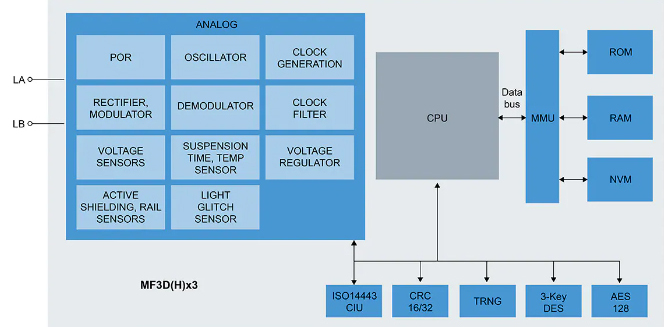
\includegraphics[width=1\linewidth]{MIFARE-DESFire-EV3.jpg}
%     \caption{DESFire EV3 block diagram}
%     \label{fig:mifare_desfire}
% \end{figure}

However, as the technologies evolve, our smartphones are also able to emulate themselves as an NFC card using Host Card Emulation (HCE)~\cite{alliance2014host}. This system is explicitly tested using an Android phone. The TransitPay application, built using React Native, used APDU commands to communicate with the Payment Operating System. The application was tested using the AID number: D2760000850101. The KHostApduServices.kt and MainApplication.kt communicate with the IoT-embedded point of sale (POS) terminal.


\subsubsection{Point Of Sale Terminal} \mbox{} \\

The Point of Sale (POS) of the TransitPay ecosystem includes different Internet of Things modules such as a microcontroller, an NFC reader, a GPS module, and a local storage module.

During the test, ESP8266 is used as the main microprocessor module. The programming is done entirely in C++ inside the Arduino Integrated Development Environment. The ESP8266 (NodeMCU) development kit is considered the microprocessor module in this system because the ESP8266 (NodeMCU), serving as the main microcontroller for the TransitPay Point of Sale, is chosen because it is inexpensive, small in form factor, meets standards as a low-power processor, and has built-in Wi-Fi capabilities. It contains the required computational resources to manage NFC reader communications, perform fare validation, maintain local data storage of transactions, and periodically communicate and synchronize with the main server/backend.~\cite{esp8266soc}.
After a successful communication with an NFC card or an emulated card, the microcontroller communicates with the NEO6M GPS module for the extraction of the longitude and the latitude of the current location. The NEO-6M GPS module is chosen due to its high accuracy, reliability, low power consumption, and ease of integration with microcontroller-based systems. It provides real-time latitude and longitude data with good positional accuracy, which is essential for location-based authentication and transaction logging in NFC-enabled systems~\cite{gpsneo6m}. 

One of the key advantages of the NEO-6M is its UART-based serial communication, which allows seamless interfacing with controllers such as ESP8266, ESP32, Arduino, and STM32 without complex protocols. The module supports the standard NMEA output format, making data parsing straightforward and lightweight, which is ideal for embedded and IoT applications with limited resources~\cite{gpsneo6m}.

% \begin{figure}
%     \centering
%     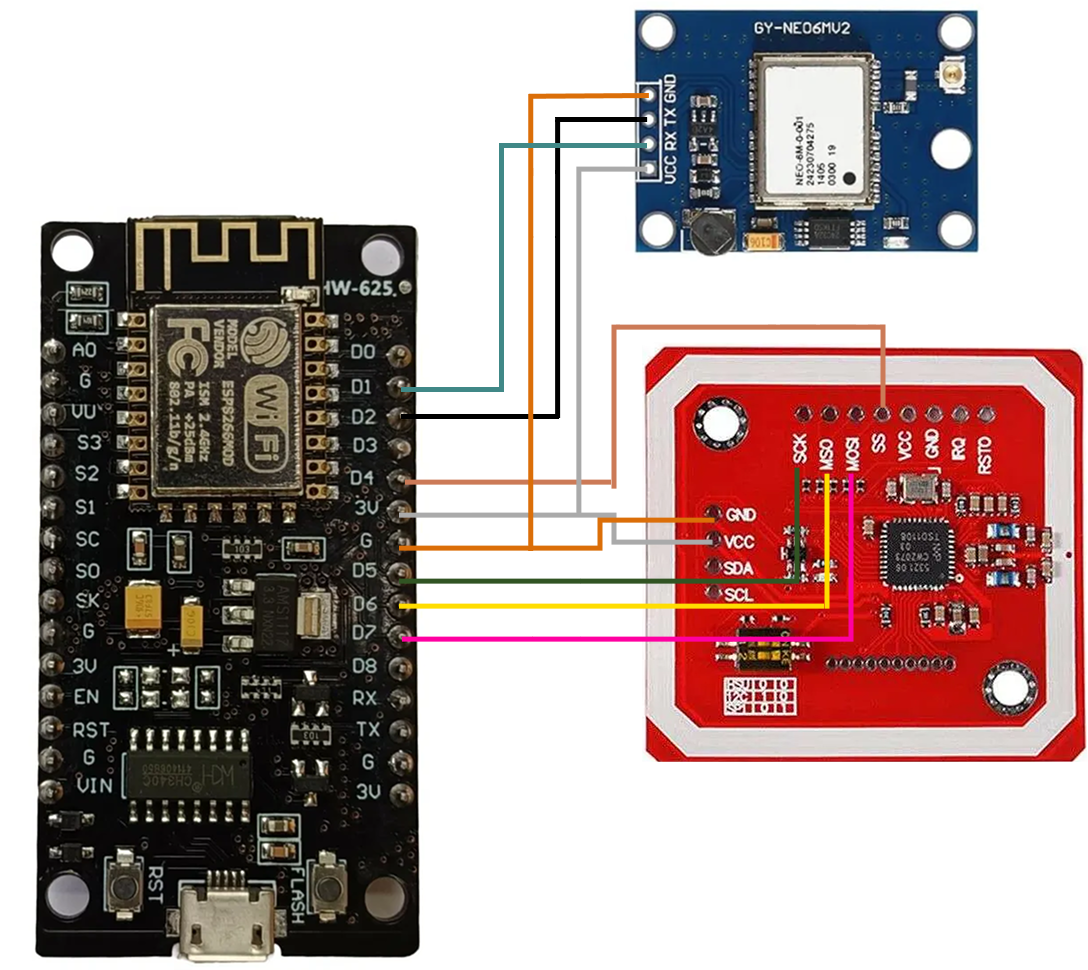
\includegraphics[width=1\linewidth]{IOT_components_wiring.png}
%     \caption{Illustration of connection of NodeMCU with PN532 and NEO-6M on SPI communication and UART communication respectively}
%     \label{fig:iot_components}
% \end{figure}

\subsubsection{Architectural Framework of the server}  \mbox{} \\

The TransitPay platform, a digital payment and transportation management solution, is powered by a strong backend system called TransitPay Server. It offers a full range of APIs for handling wallets, users, transactions, and the logistics of public transportation. It is the main hub for handling bus trips, processing NFC-based payments, and liaising with different organizational entities. It was designed with scalability and security in mind. Utilizing a cutting-edge Node.js and Express architecture, the system easily integrates with MongoDB to store persistent data.

To provide safe and precise permission management across various user roles, including administrators, ward officers, and commuters, it has an advanced Role-Based Access Control (RBAC) system. The backend also includes strong security features like rate limiting and JWT-based authentication, as well as real-time capabilities via Socket.io. This backend, which was created to support the TransitPay ecosystem, makes complicated processes like trip tracking, wallet top-ups, and card requests easier. Additionally, it ensures high availability and simplicity of integration for frontend applications and external services by offering health monitoring and a centralized entry point for multiple services.

The comprehensive details about how the fare are calculated in this system is described on a dedicated section "Fare Fare Model".

\subsubsection{The Fair Fare Model (FFM)}

The TransitPay system implements a Fair Fare Model to address the inefficiencies of fixed flat-fares, which often result in passengers overpaying for short-distance travel. This model utilizes an automated location-based mechanism to ensure that commuters are billed only for the specific stops traveled.

\textbf{Operational Mechanism}
The core logic of the model relies on a three-step transaction pipeline integrated with the vehicle's onboard IoT hardware:

\begin{enumerate}
    \item \textbf{Tap-In:} Upon boarding, the passenger taps their smartphone against the PN532 NFC module. The NEO-6M GPS module simultaneously logs the geographic coordinates of the boarding stop.
    \item \textbf{Tap-Out:} When the passenger reaches their destination and taps out, the system captures the alighting stop coordinates.
    \item \textbf{Lookup and Deduction:} The system matches the coordinate pair against a pre-loaded stop database on the ESP8266 microcontroller. The corresponding fare is retrieved from a fixed matrix and deducted instantly, requiring no manual calculation.
\end{enumerate}

\textbf{Fare Matrix Implementation}
The billing is governed by the Department of Transport Management (DoTM) guidelines. A representative sample of the Kathmandu Transit Fare Matrix (Fixed Rate) is detailed below:

\begin{table}[H]
  \centering
  \caption{Example of the fixed stop-based fare matrix}
  \label{tab:fare_matrix}
  \begin{tabular}{lccc}
    \toprule
    \textbf{From / To} & \textbf{Ratnapark} & \textbf{Lagankhel} & \textbf{Kalanki}\\
    \midrule
    \textbf{Ratnapark} & — & Rs. 30 & Rs. 35 \\
    \textbf{Lagankhel} & Rs. 30 & — & Rs. 25 \\
    \textbf{Kalanki}   & Rs. 35 & Rs. 25 & — \\
    \bottomrule
   \end{tabular}
\end{table}

By automating this process, the model eliminates revenue leakage and provides a scalable, low-cost path to digitizing transit fares.

\begin{figure*}[t]
\centering
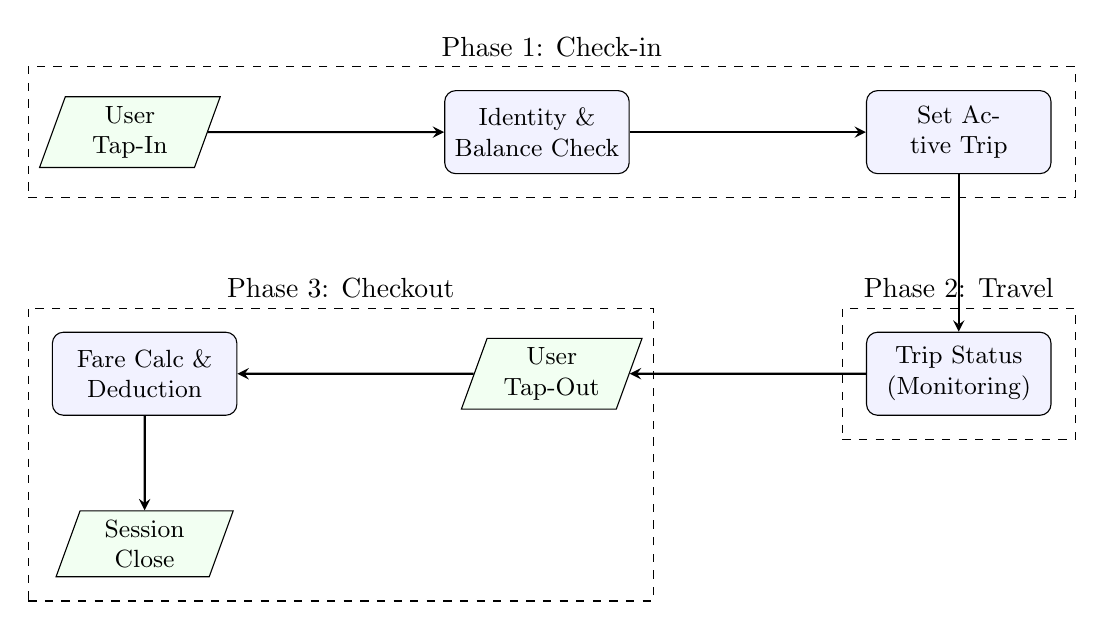
\begin{tikzpicture}[node distance=2cm and 3cm]
  % Nodes
  \node (tap) [io] {User Tap-In};
  \node (auth) [block, right=of tap] {Identity \& Balance Check};
  \node (active) [block, right=of auth] {Set Active Trip};
  
  \node (trip) [block, below=2cm of active] {Trip Status (Monitoring)};
  
  \node (exit) [io, left=of trip] {User Tap-Out};
  \node (fare) [block, left=of exit] {Fare Calc \& Deduction};
  \node (close) [io, below=1.2cm of fare] {Session Close};

  % Paths
  \draw [arrow] (tap) -- (auth);
  \draw [arrow] (auth) -- (active);
  \draw [arrow] (active) -- (trip);
  \draw [arrow] (trip) -- (exit);
  \draw [arrow] (exit) -- (fare);
  \draw [arrow] (fare) -- (close);

  % Phase Groupings (Block Structure)
  \begin{scope}[on background layer]
    \node[phase, fit=(tap)(auth)(active), label=above:Phase 1: Check-in] (p1) {};
    \node[phase, fit=(trip), label=above:Phase 2: Travel] (p2) {};
    \node[phase, fit=(exit)(fare)(close), label=above:Phase 3: Checkout] (p3) {};
  \end{scope}

\end{tikzpicture}
\caption{User flow block diagram organized by functional phases to ensure readability and logical grouping (Two-column layout).}
\label{fig:user_flow}
\end{figure*}

\subsection{Data collection and problem classification}
This section describes the analytical approach and procedures adopted to gather primary data and the systematic design approach for the classification of the problems.
\subsubsection{Data Collection} \mbox{} \\

\begin{enumerate}

\item \textbf{Research Instrument Design:} 
A structured survey questionnaire was developed to collect primary data from the target audience. The questionnaire was designed to obtain both quantitative and qualitative information regarding the challenges faced by users in the current public transportation payment system. The study adopted a mixed-method research approach to ensure comprehensive analysis of user experiences and perceptions.
\\
\\
The questionnaire consisted of:
\\
\begin{itemize}

\item \textbf{Closed-ended Questions:} 
A set of multiple-choice and Likert-scale questions were included in the survey form to obtain measurable responses regarding transportation payment issues, discount verification problems, and user acceptance of digital wallet integration.

\item \textbf{Open-ended Questions:} 
An open-ended question was included to allow respondents to describe their personal experiences related to cash handling problems, conductor payment issues, or other challenges encountered during public transportation travel.
\\
\end{itemize}

\item \textbf{Target Population and Sampling:} The survey targeted regular public transportation users including students, senior citizens, and general commuters.
\\
Approximately 29 valid responses were considered for analysis after data screening and verification.

\end{enumerate}
\subsubsection{Problem classification} \mbox{} \\
\\
From the survey analysis, several common transportation payment-related problems were identified, which justify the development of the proposed TransitPay solution. People faced different challenges while commuting in public transportation; the summarized list consists of the following:

\begin{itemize}
    \item Lack of change availability with conductors during travel
    \item Risk of overcharging or inconsistent fare collection
    \item Difficulty in verifying discount eligibility during travel
    \item Passenger discomfort during manual cash transaction inside crowded buses
    \item Limited adoption and convenience of cashless payment systems
    \\
\end{itemize}
Apart from these primary issues, the survey responses also indicated general operational and behavioral challenges associated with the current public transportation payment environment. Many users reported stress caused by manual payment handling, lack of transparency in fare calculation, and dependency on physical cash during commuting. The findings collectively suggest the necessity for a secure, automated, and user-friendly digital payment mechanism for public transportation systems.

\subsection{Testing Environment}
This section thoroughly explains the testing environment and standards of the TransitPay ecosystem, where different measures are considered as factors of tests, listly.

\begin{itemize}
    \item \textbf{Latency:} Latency is the time frame between which the user interaction and the server response is calculated. The standard of the latency in the test is the first point of interaction between the users and the output display showing success or error message.
    \item \textbf{Reliability:} Reliability describes how consistently the system performs without failures resulting in the rate of success of transactions.
    \item \textbf{Security:} This factor considers the security of the receiver (point of sale) and the sender (user), which includes the user data security and the receiver data security.
     \item \textbf{Fault Tolerance:} Fault tolerance can be defined as the ability of the system to handle the internal failures such as network connectivity issues or server downtime.
     \item \textbf{Usability: } The usability factor describes how easy or convenient it is to use the system, affecting the user experience.
\end{itemize}

\subsubsection{Routes and Fare Fare Model} \mbox{} \\

While randomly picking the testing routes inside the Kathmandu valley, the route of Machhapokhari to Ratnapark and Pulchowk to Ratnapark were choosen. So the fare matrix was also set with the stations or hubs mapped in the route.

\begin{table}[H]
\centering
\caption{Pulchowk to Ratnapark Route Fare Matrix (NPR)}
\label{tab:pulchowk_fare_matrix}
\begin{tabular}{lcccc}
\toprule
\textbf{} & \textbf{Pulchowk} & \textbf{Kupondole} & \textbf{Thapathali} & \textbf{Ratnapark} \\
\midrule
Pulchowk   & -- & 15 & 20 & 25 \\
Kupondole  & 15 & -- & 15 & 20 \\
Thapathali & 20 & 15 & -- & 20 \\
Ratnapark  & 25 & 20 & 20 & -- \\
\bottomrule
\end{tabular}
\end{table}

\begin{table*}[t]
\centering
\caption{Machhapokhari to Ratnapark Route Fare Matrix (NPR)}
\label{tab:fare_matrix}
\begin{tabular}{lcccccccc}
\toprule
\textbf{From / To} & \textbf{Machhapokhari} & \textbf{Balaju} & \textbf{Nayabazar} & \textbf{Sohrakhutte} & \textbf{Thamel} & \textbf{Lainchaur} & \textbf{Jamal} & \textbf{Ratnapark} \\
\midrule
Machhapokhari & -- & 20 & 20 & 20 & 25 & 25 & 25 & 25 \\
Balaju        & 20 & -- & 20 & 20 & 20 & 25 & 25 & 25 \\
Nayabazar     & 20 & 20 & -- & 20 & 20 & 20 & 25 & 25 \\
Sohrakhutte   & 20 & 20 & 20 & -- & 20 & 20 & 20 & 25 \\
Thamel        & 25 & 20 & 20 & 20 & -- & 20 & 20 & 20 \\
Lainchaur     & 25 & 25 & 20 & 20 & 20 & -- & 20 & 20 \\
Jamal         & 25 & 25 & 25 & 20 & 20 & 20 & -- & 20 \\
Ratnapark     & 25 & 25 & 25 & 25 & 20 & 20 & 20 & -- \\
\bottomrule
\end{tabular}
\end{table*}

\subsubsection{TransitPay sandboxed environment} \mbox{} \\
In the testing environments, the TransitPay system operates entirely within a sandboxed framework. The prototype was rigorously tested both in a controlled laboratory setting and across specific real-world public transit routes. The primary evaluations were heavily focused on Route No. 23, which served as the major testing corridor, alongside extensive deployments on the high-traffic Pulchowk to Ratnapark route to simulate complex, real-world commuting scenarios.

\subsubsection{Khalti/Esewa production environment} \mbox{} \\
For benchmarking purposes, existing digital wallets such as eSewa and Khalti were evaluated in their live production modes. These platforms rely entirely on a QR-based payment system. Because these applications are designed as general-purpose digital wallets rather than systems optimized specifically for the rapid, high-volume environment of public transportation, their performance was assessed to establish a baseline for current digital payment capabilities in transit.




\subsection{User Pipeline}
The user flow of Transitpay follows the standard NFC-based tap-to-pay system, where users are supposed to tap their payment access card into the point of sale in order to complete the transaction. In general POS, the transaction amount is set to be entered manually by the merchant. After the merchant enters the transaction amount, the user has to tap their card into the POS, and the POS connected to the server handles the payment operations. After successful verification of the payment card, the user has to wait until the POS shows the success message as output.

In TransitPay, the user provided card interacts with the POS for two different time, while entering the vehicle and while exiting the vehicle. The detailed user flow of the TransitPay system is:

\subsubsection{Phase 1 : Check-in authentication}

This phase focuses on identity verification and ensuring the user meets the minimum financial requirements to travel.

\begin{enumerate}
    \item \textbf{NFC Trigger:} While entering the bus, the users are supposed to tap their NFC-enabled entity, such as a mobile phone or NFC card, on the point of sale terminal installed on the transit.
    \item \textbf{Initial Handshake:} The POS terminal, which is equipped with an NFC reader, detects the NFC card and initiates a secure handshake with the user's device. This handshake establishes a secure communication channel between the POS and the user's device.
    \item \textbf{Balance thresold verification:} 
     \begin{itemize}
      \item The Point-of-sale terminal extracts the user's card information, including the card ID and the current balance, from the NFC card.
      \item The POS sends the user ID, timestamp and the GPS coordinates to the server.
      \item The server verifies the user's wallet balance and checks if it is sufficient to cover the minimum fare.
      \item If the user's wallet balance is sufficient, the server registers the user in a active Trip.
      \item The POS receives a success message from the server and displays a confirmation to the user to proceed.
     \end{itemize}
\end{enumerate}

\subsubsection{Phase 2 : Ongoing Trip on the transit}

\begin{enumerate}
  \item The user successfully onboarded the transit after a successful verification of the user data, exact time, and locations.
  \item Passengers or the users don't have to interact with other people verbally or physically (NFC cards) during the whole trip. 
\end{enumerate}

\subsubsection{Phase 3 : Trip Completion and Payment}
\begin{enumerate}
  \item While exiting the bus, the users are supposed to tap their NFC-enabled device, such as a mobile phone or NFC card, on the point of sale terminal installed on the transit.
  \item The POS terminal, which is equipped with an NFC reader, detects the NFC card and initiates a secure handshake with the user's device. This handshake establishes a secure communication channel between the POS and the user's device.
  \item The POS terminal extracts the user's card information, including the card ID and the current balance, from the NFC card.
  \item The POS sends the user ID, timestamp, and GPS coordinates to the server.
  \item The server verifies the user's wallet balance and checks if it is sufficient to cover the minimum fare.
  \item If the user's wallet balance is sufficient, the server registers the user in an active trip.
  \item The POS receives a success message from the server and displays a confirmation to the user to proceed.
\end{enumerate}
 \section{Cost Breakdown}
This section gives a detailed cost review and breakdown of pre-development, in-development, post-development, external or miscellaneous, and labor budgeting and costs. This section is divided into 3 different parts: production cost, labor, and miscellaneous costs.

\begin{table}[H]
  \centering
  \caption{Production Cost Breakdown}
  \label{tab:production_cost}
  \begin{tabularx}{\columnwidth}{p{5em} L r}
    \toprule
    \textbf{Particular} & \textbf{Type} & \textbf{Cost (NPR)} \\
    \midrule
    ESP8266 & Microcontroller of the point-of-sale & 800 \\
    PN532 & NFC reading/writing module & 600 \\
    NEO-6M & GPS module of the POS & 500 \\
    LCD display & Output display & 800 \\
    Case & 3D printed case & 300 \\
    NFC card & NFC entity & 250 \\
    \midrule
    \textbf{Total} & & \textbf{3000} \\
    \bottomrule
  \end{tabularx}
\end{table}



\begin{table}[H]
  \centering
  \caption{Labor Cost Breakdown}
  \label{tab:labor_cost}
  \begin{tabularx}{\columnwidth}{L r}
    \toprule
    \textbf{Particular} & \textbf{Cost (NPR/mo)} \\
    \midrule
    Development & 250,000 \\
    Hardware assembling & 300,000 \\
    \bottomrule
  \end{tabularx}
\end{table}


\begin{table}[H]
  \centering
  \caption{API Cost Breakdown}
  \label{tab:api_cost}
  \begin{tabularx}{\columnwidth}{L r}
    \toprule
    \textbf{API} & \textbf{Estimated cost} \\
    \midrule
    Google maps & NPR 1,000,000 \\
    Nagarik app API & free \\
    \midrule
    \textbf{Total} & \textbf{NPR 500,000} \\
    \bottomrule
  \end{tabularx}
\end{table}

\section{Results and interpretation }
The TransitPay system was evaluated in a controlled, sandboxed environment to assess its reliability and efficiency under different network conditions.
\subsection{Latency and Performance}
Test 1 focused specifically on speed and performance, yielding an overall success rate of 83.33\% for NFC-based transactions. 
\subsubsection{Overview} \mbox{} \\
To simulate real-world transit conditions where network connectivity can fluctuate, the transaction processing time was measured across two distinct bandwidth scenarios:

\begin{itemize}
    \item \textbf{Moderate Connectivity (6--8 Mbps):} The system demonstrated rapid processing capabilities, with recorded transaction times of 3053~ms, 2992~ms, 2406~ms, 3305~ms, 2626~ms, and 2258~ms.
    \item \textbf{Low Connectivity (2--5 Mbps):} Under constrained network speeds typical of moving vehicles passing through dead zones, the transaction times predictably increased but remained functional, recording processing times of 6297~ms, 7325~ms, and 7005~ms.
\end{itemize}

These results indicate that while the system performs optimally in standard network conditions, it maintains operational viability even when bandwidth is significantly restricted.

\subsection{Reliability and Fair Fare Model accuracy}

The ecosystem of TransitPay has not been approved by the Government of Nepal and was only tested on the sandboxed environment; one single user had to operate across two routes where the user tapped in and tapped out in different hubs.

The 


\begin{table}[H]
  \centering
  \caption{Tap-in and Tap-out hub test}
  \label{tab:tapped_in_and_tapped_out}
  \begin{tabularx}{\columnwidth}{>{\RaggedRight\arraybackslash}p{2.5cm} >{\RaggedRight\arraybackslash}X >{\RaggedRight\arraybackslash}X}
    \toprule
    \textbf{Tap-in hub} & \textbf{Tap-out hub} & \textbf{Outcome} \\
    \midrule 
    Thamel & Machhapokhari & Success (25 rupees deducted) \\
    Ratnapark & Thamel & Success (20 rupees deducted) \\
    Ratnapark & Pulchowk & Failure (Pulchowk didn't exist on Machhapokhari-Ratnapark route) \\
    Pulchowk & Ratnapark & Success (25 rupees deducted) \\
    Machhapokhari & Balaju & Failure (Geo API didn't recognize Balaju) \\
    Machhapokhari & Ratnapark & Success (24 rupees deducted) \\
    \bottomrule
  \end{tabularx}
\end{table}


\subsection{Security}

\subsection{Fault Tolerance}

\subsection{Usability}


\subsection{}

\begin{table}[H]
  \centering
  \caption{Payment System Performance Comparison}
  \label{tab:comparison}
  \begin{tabularx}{\columnwidth}{>{\RaggedRight\arraybackslash}p{2.5cm} >{\RaggedRight\arraybackslash}X >{\RaggedRight\arraybackslash}X}
    \toprule
    \textbf{Factor} & \textbf{TransitPay} & \textbf{Esewa/Khalti QR} \\
    \midrule
    Method & NFC device Tap in and tap out & the receiver's QR scanned by User's device \\
        
    Reliability & 83.33\% success rate on 6 Mbps average internet speed & 100\% success rate on 8 Mbps average internet speed \\
    
    Latency & 3 seconds average from user's interaction to server response & 35 seconds average from user's interaction to server response \\
    
    Fault tolerance & Uses local queuing for connectivity issues. & Direct failure (no uptime services) \\

    User connectivity & Not necessary & very essential to use services \\

    POS Security & Encrypted communication only (no data exposed) & QR code can be decoded and not encrypted (data exposed) \\

    User data security & 100\% encrypted communication with APDU & industry-level standards for the user data protection.\\

    
    
    \bottomrule
  \end{tabularx}
\end{table}

\begin{figure}[H]
\centering
\label{fig:performance_bar}

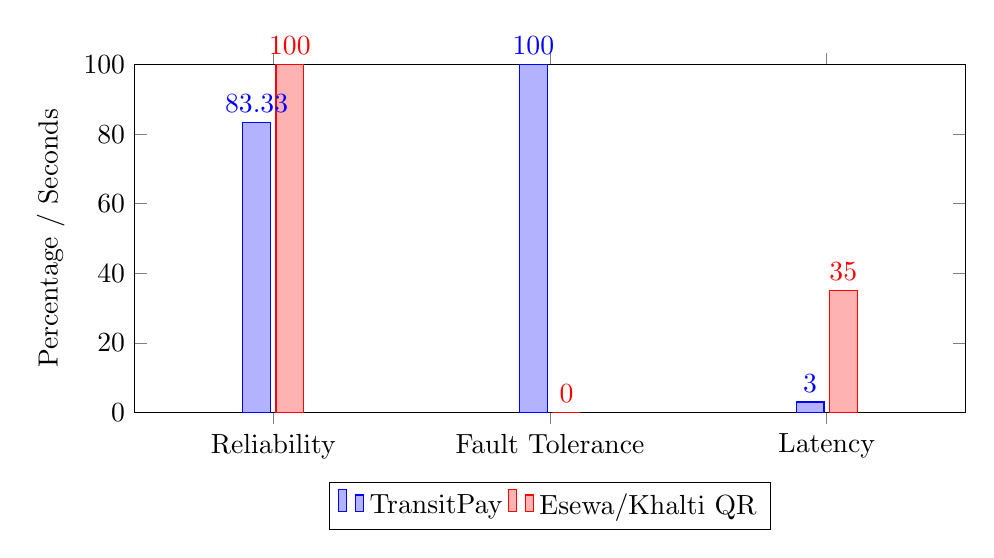
\begin{tikzpicture}
\begin{axis}[
    ybar,
    bar width=10pt,
    width=\columnwidth,
    height=6cm,
    ymin=0,
    ymax=100,
    ylabel={Percentage / Seconds},
    symbolic x coords={Reliability, Fault Tolerance, Latency},
    xtick=data,
    legend style={at={(0.5,-0.2)}, anchor=north, legend columns=-1},
    nodes near coords,
    enlarge x limits=0.25
]

\addplot coordinates {(Reliability,83.33) (Fault Tolerance,100) (Latency,3)};
\addplot coordinates {(Reliability,100) (Fault Tolerance,0) (Latency,35)};

\legend{TransitPay, Esewa/Khalti QR}

\end{axis}
\end{tikzpicture}
\caption{Performance Comparison of TransitPay and QR-based Payments}

\end{figure}

\subsection{Alignment Between Identified Problems and Proposed Solutions}

\section{Discussions}


\section{Limitations}
\subsection{Cross-platform availability of host card emulation.}

\section{Conclusion}




%%
%% The acknowledgments section is defined using the "acks" environment
%% (and NOT an unnumbered section). This ensures the proper
%% identification of the section in the article metadata, and the
%% consistent spelling of the heading.
\begin{acks}
To Sunway College Kathmandu Innovation Lab, for providing the IoT based equipments and platform like Codarambha to built an MVP.
\end{acks}

%%
%% The next two lines define the bibliography style to be used, and
%% the bibliography file.
\bibliographystyle{ACM-Reference-Format}
\bibliography{sample-base}

%%
%% If your work has an appendix, this is the place to put it.
\appendix

% \section{Research Methods}

% \subsection{Part One}

% Lorem ipsum dolor sit amet, consectetur adipiscing elit. Morbi
% malesuada, quam in pulvinar varius, metus nunc fermentum urna, id
% sollicitudin purus odio sit amet enim. Aliquam ullamcorper eu ipsum
% vel mollis. Curabitur quis dictum nisl. Phasellus vel semper risus, et
% lacinia dolor. Integer ultricies commodo sem nec semper.

% \subsection{Part Two}

% Etiam commodo feugiat nisl pulvinar pellentesque. Etiam auctor sodales
% ligula, non varius nibh pulvinar semper. Suspendisse nec lectus non
% ipsum convallis congue hendrerit vitae sapien. Donec at laoreet
% eros. Vivamus non purus placerat, scelerisque diam eu, cursus
% ante. Etiam aliquam tortor auctor efficitur mattis.

% \section{Online Resources}

% Nam id fermentum dui. Suspendisse sagittis tortor a nulla mollis, in
% pulvinar ex pretium. Sed interdum orci quis metus euismod, et sagittis
% enim maximus. Vestibulum gravida massa ut felis suscipit
% congue. Quisque mattis elit a risus ultrices commodo venenatis eget
% dui. Etiam sagittis eleifend elementum.

% Nam interdum magna at lectus dignissim, ac dignissim lorem
% rhoncus. Maecenas eu arcu ac neque placerat aliquam. Nunc pulvinar
% massa et mattis lacinia.

\end{document}
\endinput
%%
%% End of file `sample-sigconf.tex'.
